\section{Results}\label{sec:results}
In this section, we use CMC to estimate posterior parameter distributions for three biological systems. In all but one of the examples, we assume that the first step of CMC (``SnapshotEstimator'' within Algorithm \ref{alg:cmc}) has already been completed, and we are faced with inferring a parameter distribution which, when mapped to outputs, recapitulates the target density. To accompany the text, we provide the Julia notebook used to generate the results. A table of priors used for each example is provided in Table \ref{tab:priors}.


\subsection{Growth factor model}
We first consider the ``growth factor model'' introduced by \cite{dixit2018maximum}, which concerns the dynamics of inactive ligand-free cell surface receptors, $R$, and active ligand-bound cell surface receptors, $P$, modulated by an exogenous ligand, $L$. The governing dynamics are determined by the following system,
%
\begin{align}\label{eq:growth_factor}
\frac{dR}{dt} &= R_T k_{deg} + k_1 L R(t) + k_{-1} P(t) - k_{deg} R(t)\\
\label{eq:growth_factor1}
\frac{dP}{dt} &= k_1 L R(t) - k_{-1} P(t) - k^*_{deg} P(t),
\end{align}
with initial conditions,
\begin{equation*}
R(0) = 0.0, \qquad P(0) = 0.0,
\end{equation*}
%
where $\boldsymbol{\theta}=(R_T, k_1, k_{-1}, k_{deg}, k^*_{deg})$ are parameters to be determined. In this example, we use measurements of the active ligand-bound receptors $P$ to estimate cellular heterogeneity in these processes. We denote the solution of eq. (\ref{eq:growth_factor1}) as $P(t; \boldsymbol{\theta}, L)$. \textcolor{blue}{Here we generate a target model by forward simulations of eq. \eqref{eq:growth_factor}; in each case recording $(P(10; \boldsymbol{\theta}, 2), P(10; \boldsymbol{\theta}, 10))$. In each forward simulation, we fix $(k_{-1}, k_{deg}, k^*_{deg}) = (8, 0.015, 0.25)$ and independently sample values $R_T\sim \mathcal{N}(6.5\times 10^5, 0.6\times 10^4)$ and $k_1\sim \mathcal{N}(1.7, 0.05)$. This generates an output distribution approximately given by,}
%
\begin{equation}\label{eq:MM_outputDistribution}
\boldsymbol{q} =
\begin{pmatrix}
q_1\\
q_2\\
\end{pmatrix}
=
\begin{pmatrix}
P(10; \boldsymbol{\theta}, 2)\\
P(10; \boldsymbol{\theta}, 10)\\
\end{pmatrix} \sim  \mathcal{N}
\begin{bmatrix}
\begin{pmatrix}
2\times 10^4\\
3\times 10^4\\
\end{pmatrix}, \;\;
\begin{pmatrix}
1\times 10^5 & 0\\
0 & 1\times 10^5\\
\end{pmatrix}
\end{bmatrix}.
\end{equation}
%

\subsubsection{Uniform prior}\label{sec:growthmodel_uniform}
For an under-determined model, the number of QOIs, $m$, is less than the number of parameters, $p$, and there typically exists a non-singular set of parameter distributions mapping to the same target output distribution. To uniquely identify a posterior parameter distribution, it is, therefore, necessary to specify a prior parameter distribution. By incorporating priors, this allows pre-existing biological knowledge to be included, leading to reduced uncertainty in parameter estimates. CMC allows any prior with correct support to be used. Changes to priors affect both the ``ContourVolumeEstimation'' and ``MCMC'' steps of CMC (Algorithm \ref{alg:cmc}), so that the (changed) posterior parameter distribution still maps to the target.

To start, we specify a uniform prior for each of the five parameters, with bounds given in Table \ref{tab:priors}, and use CMC to estimate the posterior parameter distribution. In Figure \ref{fig:growth_factor_outputs}A, we show the sampled outputs (blue points) versus the contours of the target distribution (black solid closed curves), illustrating a good correspondence between the sampled and target densities. Above and to the right of the main panel, we also display the marginal target densities (solid black lines) versus kernel density estimator reconstructions of the output marginals from the CMC samples (dashed blue lines), which again highlights the fidelity of the CMC sampled density to the target.

\begin{figure}[H]
	\centerline{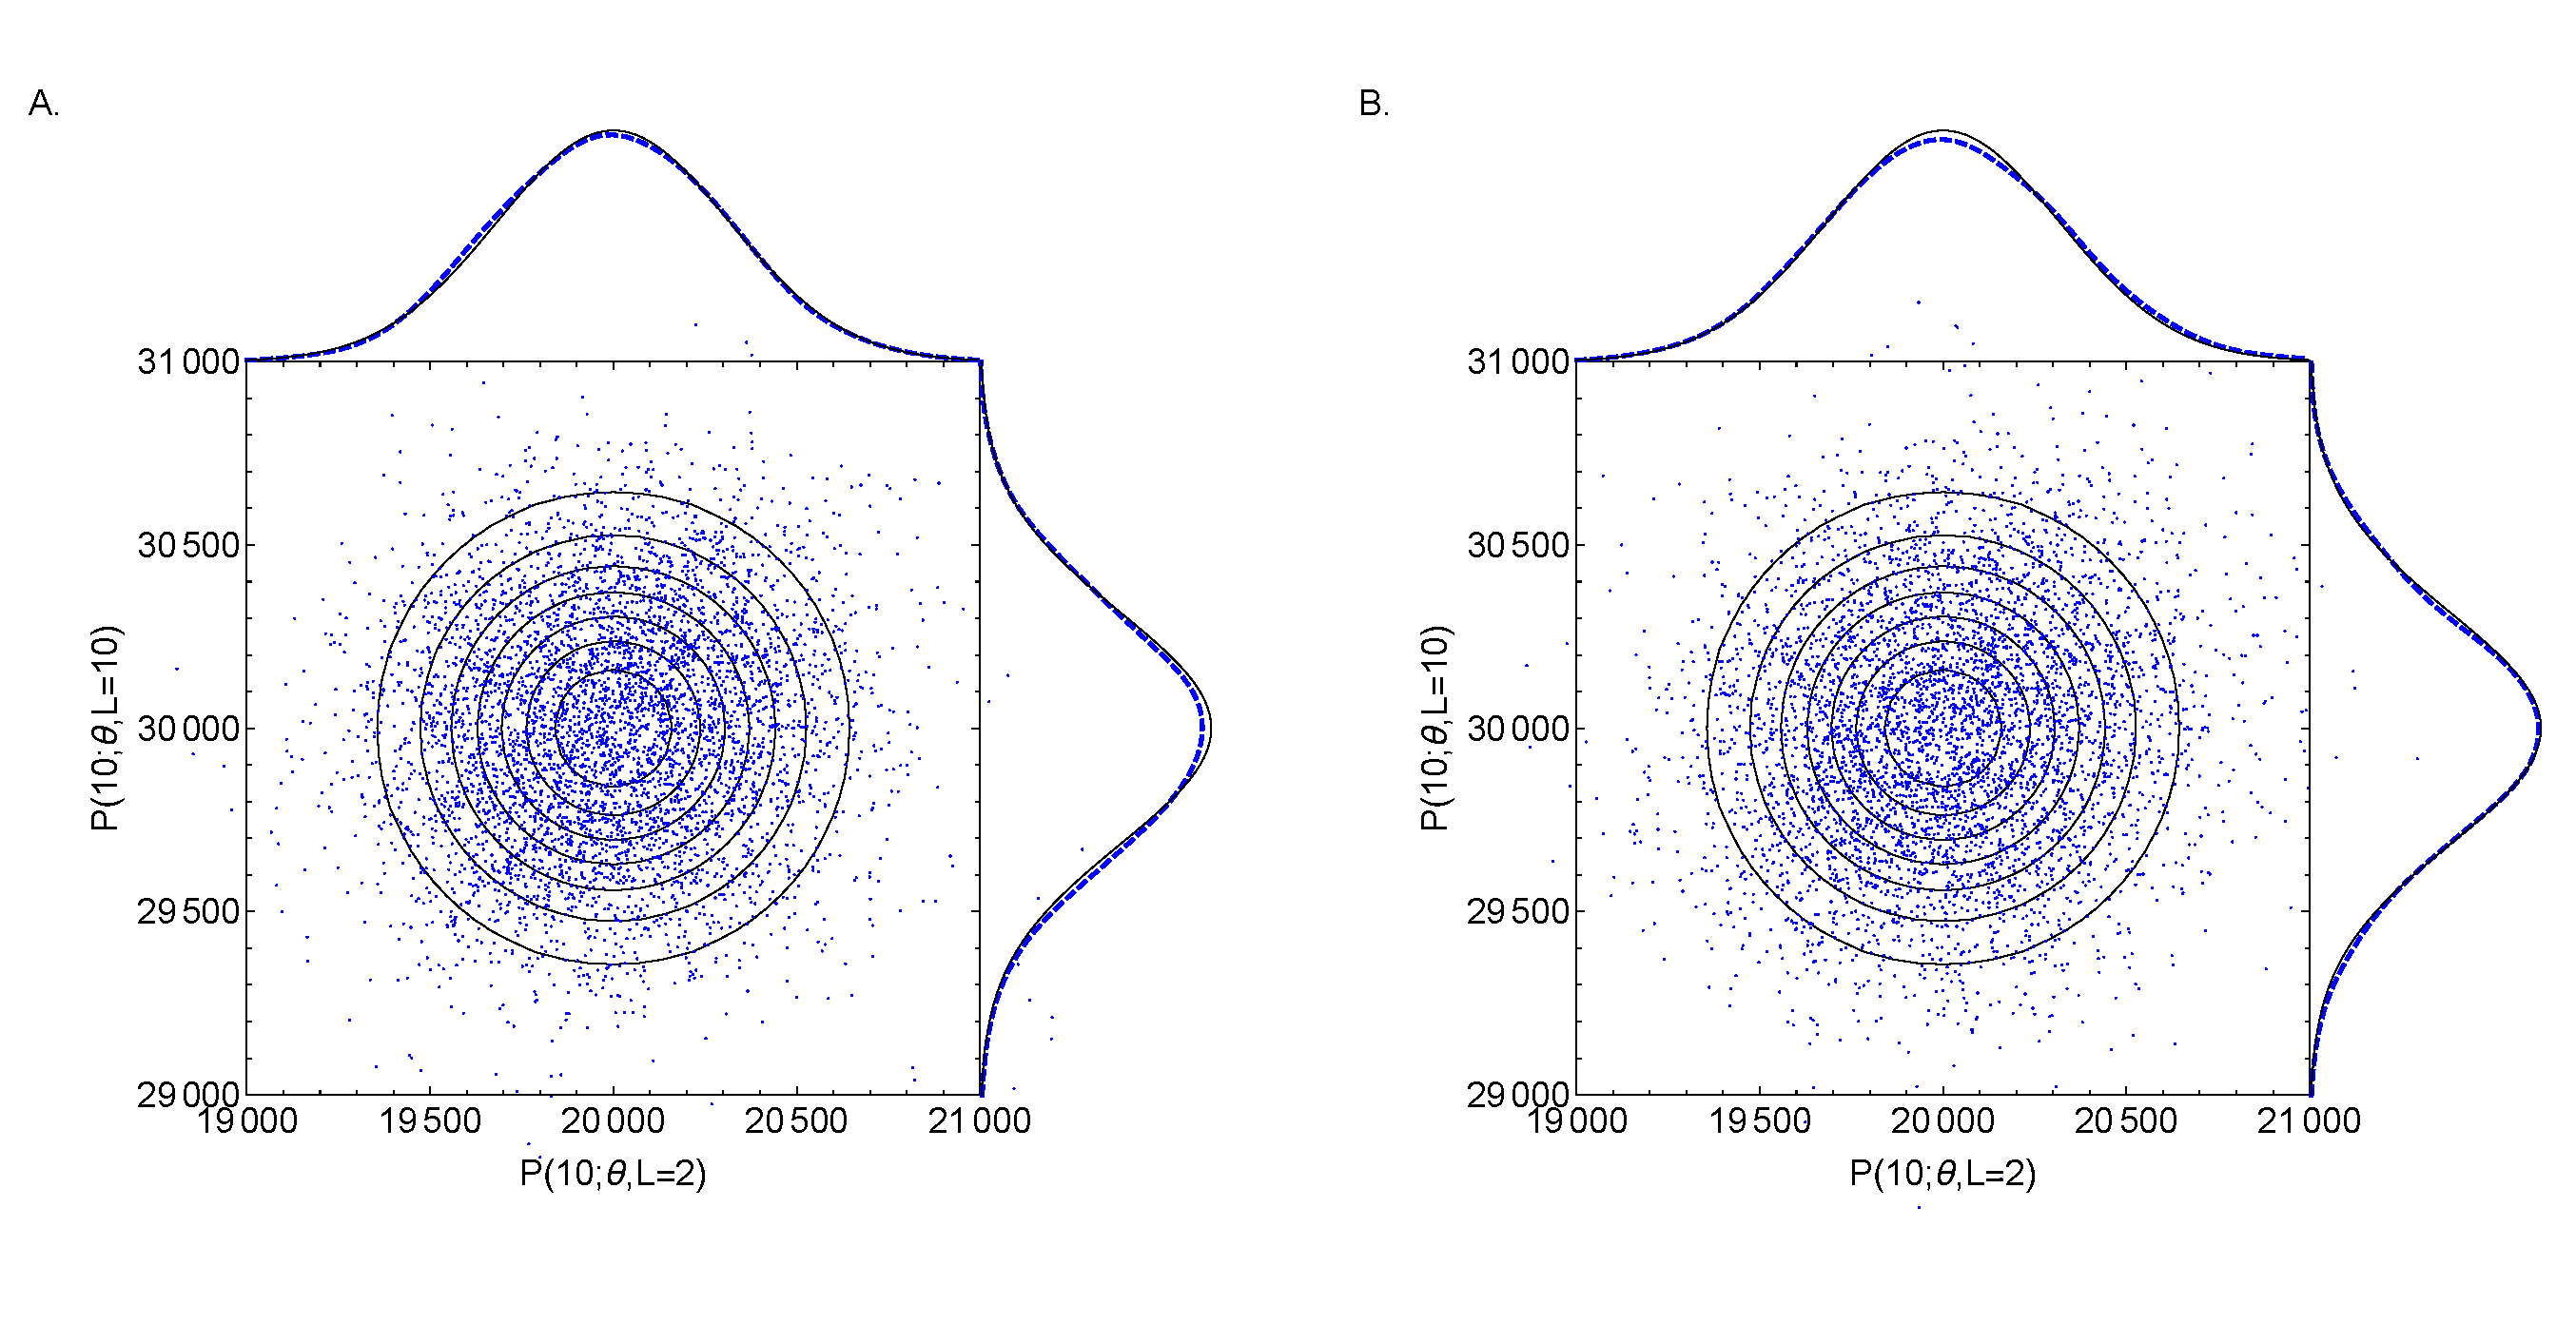
\includegraphics[width=\textwidth]{../figures/growth_factor_outputs.pdf}}
	\caption{\textbf{Growth factor model. Target joint output distribution (solid contour lines) and target marginal distributions (solid lines; above and to the right of each figure) versus outputs sampled by CMC (blue points) and reconstructed marginals (dashed lines). (A) uniform priors. (B) Gaussian priors.} In CMC, 100,000 independent samples were used in the ``ContourVolumeEstimator'' step and 10,000 MCMC samples across each of 4 Markov chains were used in the second step, with the first half of the chains discarded as ``warm-up'' \cite{lambert2018Student}. For the reconstructed marginal densities in the plots, we use Mathematica's ``SmoothKernelDistribution'' function specifying bandwidths of 100 with Gaussian kernels \cite{mathematica}.}
	\label{fig:growth_factor_outputs}
\end{figure}


In Figure \ref{fig:growth_factor_inputs}A, we plot the joint posterior parameter distribution for $k_1$, the rate of ligand binding to inactive receptors and $k_{-1}$, which dictates the rate of the reverse reaction. A given level of bound ligands can be generated in many different ways. Not surprisingly, it is the \emph{ratio} of the forward and reverse reaction rates, $k_1$ and $k_{-1}$ respectively, that is of greatest importance, and because of this, the distribution representing cell process heterogeneity contains linear positive correlations between these parameters.


In Figure \ref{fig:growth_factor_inputs}B, we show the posterior parameter distribution for $k_{deg}$, the rate of degradation of ligand-free cell surface receptors and $R_T$, the rate of introduction of ligand-free cell surface receptors. This plot shows more concentrated posterior mass than in Figure \ref{fig:growth_factor_inputs}A.


Why do our measurements allow us to better resolve $(k_{deg},R_T)$ compared to $(k_1,k_{-1})$? To answer this, it is useful to calculate the sensitivity of $P(t; \boldsymbol{\theta}, L)$ to changes in each of the parameters. To account for the differing magnitudes of each parameter, we calculate elasticities, the proportional changes in measured output for a proportional change in parameter values, using the forward sensitivities method described in \cite{DGCT2018}, and these are shown in Figure \ref{fig:dixit_elasticities}. When the exogenous ligand is set at $L=2$, these indicate the active ligand-bound receptor concentration is most elastic to changes in $R_T$ and $k_{deg}$. This higher elasticity means that their range is more restricted by the output measurement than for $k_1$ and $k_{-1}$, which have much smaller elasticities at $t=10$. In Table \ref{tab:growth_factor_results}, we show the posterior quantiles for the estimated parameters, and in the last column, indicate the ratio of the 25\%-75\% posterior interval widths to the uniform prior range for each parameter. These were strongly negatively correlated with the magnitude of the elasticities for each parameter ($\rho=0.95$, $t=-5.22$, $df=3$, $p=0.01$ for Pearson's product-moment correlation), indicating the utility of sensitivity analyses for optimal experimental design, \textcolor{blue}{see e.g., \cite{Banks2011}}. We suggest, however, that CMC can also be used for this purpose. If an experimenter generates synthetic data for various choices of QOIs, they can use CMC to derive the posterior parameter distributions in each case. They then, simply, select the particular QOI producing the narrowest posterior for key parameters.

\textcolor{blue}{In both panels of Figure \ref{fig:growth_factor_inputs}, we also plot the ``\textit{actual}'' parameter values as dashed lines: for $k_{-1}$ and $k_{deg}$, these indicate the true (fixed) parameter values, and, for $k_1$ and $R_T$, they show the mean of each Gaussian sampling distributions ($\pm$ two standard deviations shown by shaded rectangles). For most parameters, these indicate that the area of highest posterior density is close to the causative parameter values. This is reaffirmed in the top panel of Table \ref{tab:growth_factor_results}, where, in all cases, the actual parameter values lie within the estimated 95\% quantiles for each parameter -- indicating that the parameters were reasonably well identified.}


\begin{figure}[H]
	\centerline{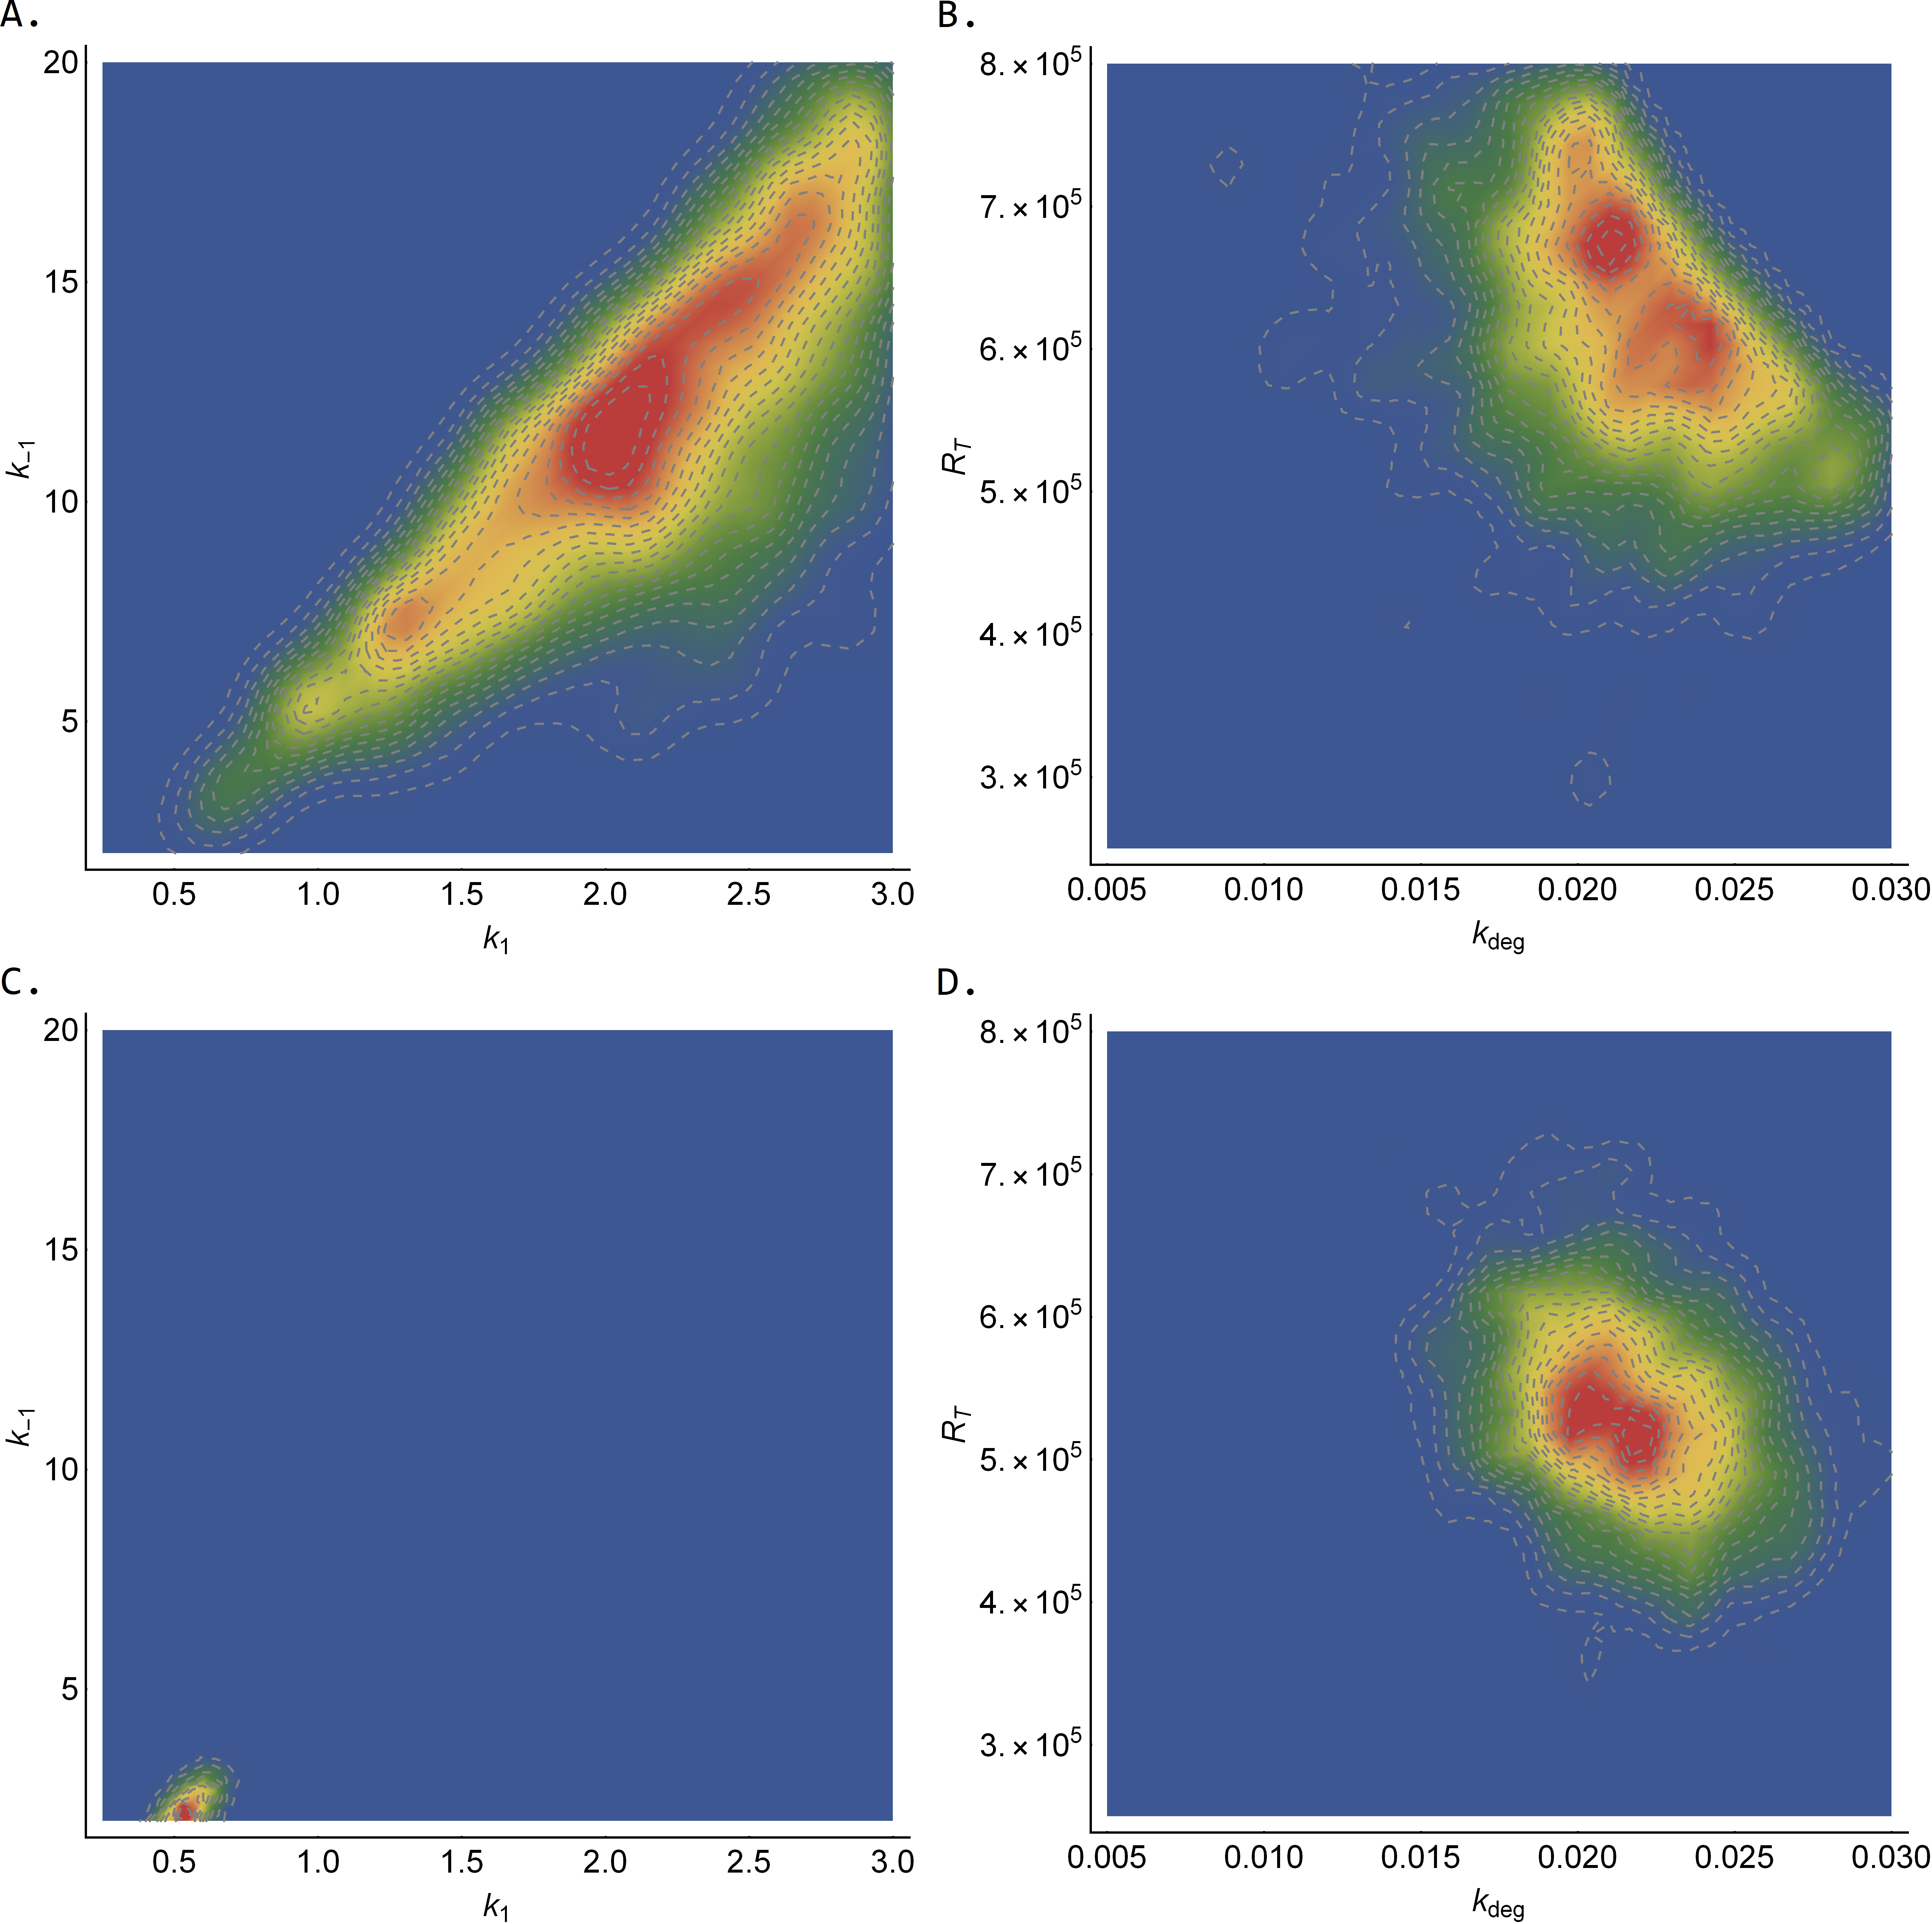
\includegraphics[width=\textwidth]{../figures/growth_factor_inputs.pdf}}
	\caption{\textbf{Growth factor model. Joint posterior distributions estimated by CMC. Top row (A-B): $(k_1,k_{-1})$ and $(k_{deg},R_T)$ using uniform priors. Bottom row (C-D): $(k_1,k_{-1})$ and $(k_{deg},R_T)$ using Gaussian priors.} \textcolor{blue}{In all panels, dashed lines indicate the parameter set or distribution used to generate the target distribution given by eq. \eqref{eq:MM_outputDistribution}: for $k_{-1}$ and $k_{deg}$, the dashed lines show true parameter values and for $k_1$ and $R_T$, they show the mean of each Gaussian sampling distributions ($\pm$ two standard deviations shown by shaded rectangles).} See Figure \ref{fig:growth_factor_outputs} caption for CMC details and Table \ref{tab:priors} for the priors used. Red (blue) indicates areas of relatively high (low) probability density.}
	\label{fig:growth_factor_inputs}
\end{figure}

\begin{figure}[H]
	\centerline{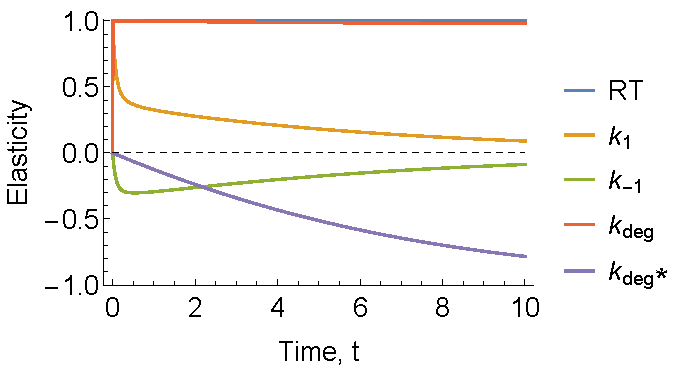
\includegraphics[width=0.7\textwidth]{../figures/dixit_elasticities.pdf}}
	\caption{\textbf{Growth factor model. Elasticities of the active ligand-bound receptors $P$ with respect to each parameter as a function of time.} When calculating the elasticities of each parameter, the other parameters were set to their posterior medians given in Table \ref{tab:growth_factor_results} and $L=2$.}
	\label{fig:dixit_elasticities}
\end{figure}

\subsubsection{Gaussian prior}
We now use CMC to estimate the posterior parameter distribution, when using Gaussian priors (prior hyperparameters shown in Table \ref{tab:priors}), which are more concentrated than the uniform priors used in \S\ref{sec:growthmodel_uniform}. As desired, the target output distribution appears virtually unaffected by the change of priors (Figure \ref{fig:growth_factor_outputs}B) although with substantial changes to the posterior parameter distribution (Figure \ref{fig:growth_factor_inputs}C and \ref{fig:growth_factor_inputs}D). In particular, the marginal posterior distributions obtained from the Gaussian prior are narrower compared to the uniform case (rightmost column of Table \ref{tab:growth_factor_results}).

As in traditional Bayesian inference, prior choice has a greater influence on the posterior distribution when data provide less information on the underlying process. This is readily apparent in comparing the dramatic change from Figure \ref{fig:growth_factor_outputs}A to \ref{fig:growth_factor_outputs}C for $(k_1,k_{-1})$, which have low sensitivities, with the more nuanced change from Figure \ref{fig:growth_factor_outputs}B to \ref{fig:growth_factor_outputs}D for $(k_{deg},R_T)$, which have high sensitivities. \textcolor{blue}{The results also indicate the bias-variance trade-off inherent in Bayesian analysis: when relatively uninformative priors are specified (Figure \ref{fig:growth_factor_outputs}A\&B), the posterior distributions are wider but their centre lies, in general, closer to the true values (dashed lines) than when more information is included in the priors (Figure \ref{fig:growth_factor_outputs}C\&D).}

\begin{table}
	\scriptsize
\begin{tabular}{c|ccccc|c|c}
\toprule
&&&&&&&                                         Posterior \\
Parameter &  \multicolumn{5}{c}{Quantiles} &&  25\%-75\% \\
          & 2.5\% & 25\% & 50\% & 75\% & 97.5\% & True values & conc.\\
\toprule
\multicolumn{8}{c}{Uniform prior} \\
\toprule
$R_T$       &  441,006 & 548,275 & 606,439 & 677,055 & 772,484 & 650,000 & 23\%\\
$k_1$       &  0.90 & 1.69 & 2.17 & 2.56 & 2.95 & 1.70 & 32\%\\
$k_{-1}$    & 4.35 & 8.35 & 11.23 & 14.23 & 18.71 & 8.00 & 33\%\\
$k_{deg}$   & 0.013 & 0.019 & 0.021 & 0.024 & 0.029 & 0.015 & 20\%\\
$k^*_{deg}$ & 0.20 & 0.34 & 0.40 & 0.44 & 0.49 & 0.25 & 27\%\\
\toprule
\multicolumn{8}{c}{Gaussian prior} \\
\toprule
$R_T$       & 408,396 & 487,372 & 529,558 & 577,970 & 678,632 & 650,000 & 16\%\\
$k_1$       & 0.39 & 0.49 & 0.54 & 0.60 & 0.70 & 1.70 & 4\%\\
$k_{-1}$    & 1.39 & 1.92 & 2.26 & 2.63 & 3.35 & 8.00 & 4\%\\
$k_{deg}$   & 0.016 & 0.020 & 0.022 & 0.024 & 0.027 & 0.015 & 16\%\\
$k^*_{deg}$ & 0.22 & 0.29 & 0.33 & 0.38 & 0.46 & 0.25 & 21\%\\
\end{tabular}
\caption{\textbf{Growth factor model. Estimated quantiles from CMC samples with uniform and Gaussian priors.} The last column indicates the proportion of the uniform prior bounds occupied by the 25\%-75\% posterior interval in each case. The prior hyperparameters used in each case are given in Table \ref{tab:priors}.}
\label{tab:growth_factor_results}
\end{table}

\subsection{Michaelis-Menten kinetics}
In this section, we use CMC to invert output measurements from the Michaelis-Menten model of enzyme kinetics (see, for example, \cite{murray2007mathematical}) - illustrating how CMC can determine resolve population substructure from a multimodal output distribution. The Michaelis-Menten model of enzyme kinetics describes the dynamics of concentrations of an enzyme, $E$, a substrate, $S$, an enzyme-substrate complex, $C$, and a product, $P$,
%
\begin{equation}\label{eq:michaelis_menten}
\begin{aligned}
\frac{dE}{dt} &= -k_f E(t)S(t) + k_r C(t) + k_{cat} C(t), \\
\frac{dS}{dt} &= -k_f E(t)S(t) + k_r C(t), \\
\frac{dC}{dt} &= \phantom{-}k_f E(t)S(t) - k_r C(t) - k_{cat} C(t), \\
\frac{dP}{dt} &= \phantom{-}k_{cat} C(t),
\end{aligned}
\end{equation}
%
with initial conditions,
\begin{equation}
E(0) = E_0, \; S(0)=S_0, \; C(0)=C_0, \; P(0)=P_0,
\end{equation}
%
where $k_f$ is the rate of the forward reaction $E+S \rightarrow C$, $k_r$ is the rate of the reverse reaction $C \rightarrow E+S$, and $k_{cat}$ is the catalytic rate of product formation by the reaction $C \rightarrow E + P$.


\subsubsection{Bimodal output distribution}
When subpopulations of cells, each with distinct dynamics, are thought to exist, determining their characteristics - the proportions of cells in each cluster, their distinct parameter values, and so on - is often of key interest \cite{hasenauer2011identification,loos2018hierarchical}. Before formal inference occurs, an output distribution with multiple modes may signal the existence of fragmented subpopulations of cells, and to exemplify this, we target a bimodal bivariate Gaussian distribution for measurements of the level of enzyme and substrate at $t=1$ and $t=2$ respectively,
%
\begin{equation}
\begin{gathered}\begin{aligned}
\boldsymbol{q} = \begin{pmatrix} q_1 \\ q_2 \end{pmatrix}
 = \begin{pmatrix} E(2.0; \boldsymbol{\theta}) \\ S(1.0; \boldsymbol{\theta}) \end{pmatrix}
&  \sim
p(\boldsymbol{q}; \boldsymbol{\mu}_1,\Sigma_1, \boldsymbol{\mu}_2, \Sigma_2) \\
&= \frac{1}{2}\left(\mathcal{N}(\boldsymbol{q}; \boldsymbol{\mu}_1,\Sigma_1)
+ \mathcal{N}(\boldsymbol{q}; \boldsymbol{\mu}_2,\Sigma_2)\right),
\end{aligned}\end{gathered}
\end{equation}
%
where $\boldsymbol{\theta}=(k_f,k_r,k_{cat})$. The parameters of the Gaussian mixture components are,
%
\begin{equation*}
\begin{aligned}
&\boldsymbol{\mu}_1=\begin{pmatrix} 2.2 \\ 1.6 \end{pmatrix} , \; \Sigma_1
                   =\begin{pmatrix} 0.018 & -0.013 \\ -0.013 & 0.010 \end{pmatrix}, \\
&\boldsymbol{\mu}_2=\begin{pmatrix} 2.8 \\ 1.0 \end{pmatrix}, \; \Sigma_2
                   =\begin{pmatrix} 0.020 & -0.010 \\ -0.010 & 0.020 \end{pmatrix}.
\end{aligned}
\end{equation*}
%
In what follows, we specify uniform priors on each element of $\boldsymbol{\theta}$ (see Table \ref{tab:priors}). Using a modest number of samples in each step, CMC provides a close approximation to the output target distribution (Figure \ref{fig:mm_bimodal_inputs_outputs}A). Without providing \textit{a priori} information on the subpopulations of cells, two distinct clusters of cells emerged from application of CMC (orange and blue points in Figure \ref{fig:mm_bimodal_inputs_outputs}B) - each corresponding to distinct modes of the output distribution (corresponding coloured points in Figure \ref{fig:mm_bimodal_inputs_outputs}A). It is worth noting, however, that the issues inherent with using MCMC to sample multimodal distributions similarly apply here. So, whilst adaptive MCMC \cite{johnstone2016uncertainty} sufficed to explore this posterior surface, it may be necessary to use MCMC methods more robust to such geometries in other cases (for example, population MCMC \cite{jasra2007population}).

\begin{figure}[H]
\centerline{\includegraphics[width=\textwidth]{../figures/mm_bimodal_inputs_outputs.pdf}}
\caption{\textbf{Michaelis-Menten model. (A) Bimodal target distribution $\boldsymbol{q}$ (solid contour lines) versus output samples (points). (B) posterior parameter samples (points).} The solid and dashed lines above and to the side of panel A indicate the target and estimated marginal output distributions, respectively. In B, only estimated parameter marginals are shown as the exact solutions are unknown. The orange (blue) points in A were generated by the orange (blue) parameter samples in B. See Figure \ref{fig:growth_factor_outputs} caption for CMC details. Mathematica's ``SmoothKernelDistribution'' function \cite{mathematica} with Gaussian kernels was used to construct marginal densities with: (A) default bandwidths, and (B) bandwidths of 0.3 (horizontal axis) and 0.03 (vertical axis). Mathematica's ``ClusteringComponents'' function \cite{mathematica} was used to identify clusters
in B.}
\label{fig:mm_bimodal_inputs_outputs}
\end{figure}

\subsubsection{Four-dimensional output distribution}
Loos et al. (2018) consider a multidimensional output distribution, with correlations between system characteristics that evolve over time. Our approach allows arbitrary covariance structure between measurements, and to exemplify this, we now target a four-dimensional output distribution, with paired measurements of enzyme and substrate at $t=1$ and $t=2$,
%
\begin{equation}\label{eq:MM_4d_output}
\begin{aligned}
\boldsymbol{q} = \begin{pmatrix} q_1 \\ q_2 \\ q_3 \\ q_4 \end{pmatrix} &=
\begin{pmatrix}
E(1.0; \boldsymbol{\theta})\\
S(1.0; \boldsymbol{\theta})\\
E(2.0; \boldsymbol{\theta})\\
S(2.0; \boldsymbol{\theta})\\
\end{pmatrix}
\\
&\sim  \mathcal{N}
\begin{bmatrix}
\begin{pmatrix}
0.5\\
2.8\\
0.9\\
1.4\\
\end{pmatrix}, \;\;
\begin{pmatrix}
0.02 &  -0.05 &  0.04 & -0.05\\
-0.05 & 0.30  & -0.15 & 0.20\\
0.04 & -0.15  & 0.12  &  -0.17\\
-0.05 & 0.20 & -0.17 & 0.30
\end{pmatrix}
\end{bmatrix}.
\end{aligned}
\end{equation}
%
Since this target has four QOIs, and the Michaelis-Menten model has three rate parameters $(k_f,k_r,k_{cat})$, the system is over-identified and so CMC cannot be straightforwardly applied. Instead, we allow the four initial states $(E_0, S_0, C_0, P_0)$ to be uncertain quantities, bringing the total number of parameters to seven. We set uniform priors on all parameters (see Table \ref{tab:priors}). In order to check that the model and priors were consistent with the output distribution given by eq. (\ref{eq:MM_4d_output}), we plotted the output measurements used to estimate contour volumes (obtained from the first step of the ``ContourVolumeEstimator'' method in Algorithm \ref{alg:cmc}) against the target (Figure \ref{fig:mm_4d_main}). Since the main support of the densities (black contours) lies within a region of output space reached by independent sampling of the priors (blue points), this indicated the target could feasibly be generated from this model and priors, and we proceeded to estimation by CMC.

\begin{figure}[H]
  \centerline{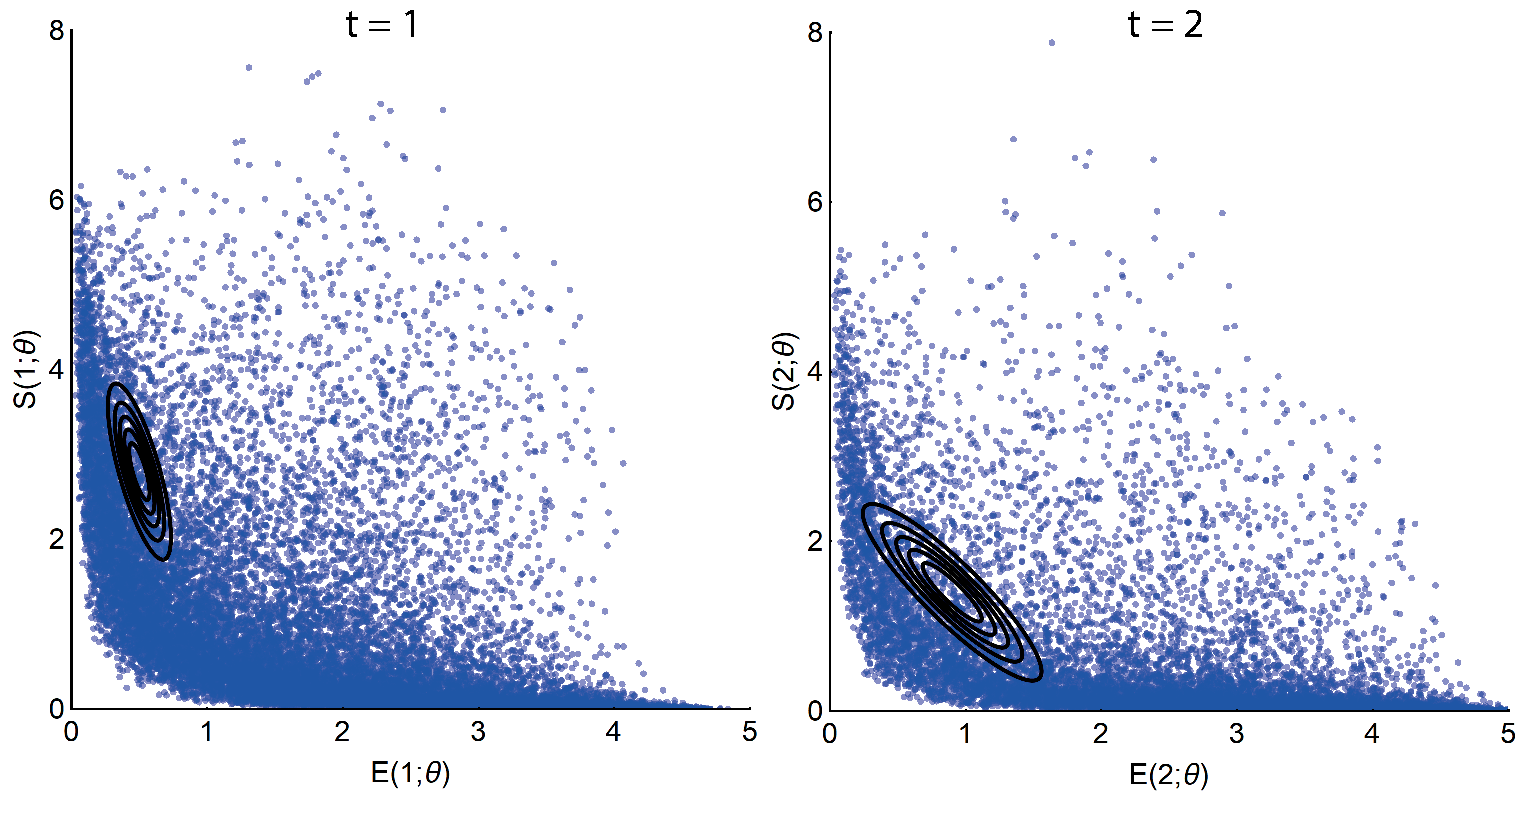
\includegraphics[width=\textwidth]{../figures/mm_4d_main.pdf}}
  \caption{\textbf{Michaelis-Menten model. QOIs (blue points) obtained by independently sampling the priors versus the target distribution (black solid contours). Left: $(q_1,q_2)$. Right: $(q_3,q_4)$.} We show 20,000 output samples, where each set of four measurements was obtained from a single sample of all parameters. The output target distribution shown by the contours corresponds to the marginal densities of each pair of enzyme-substrate measurements given by eq. (\ref{eq:MM_4d_output}).}
  \label{fig:mm_4d_main}
\end{figure}

Figure \ref{fig:mm_4d_outputs} plots the output samples of enzyme and substrate from the last step of CMC for $t=1$ (blue points) and $t=2$ (orange points) versus the contours (black lines) of the joint marginal distributions of eq. (\ref{eq:MM_4d_output}). The distribution of paired enzyme-substrate samples illustrates that the CMC output distribution closely approximates the target density, itself representing dynamic evolution of the covariance between enzyme and substrate measurements. Target marginal distributions (solid lines) along with their approximations from kernel density estimation (dashed lines) are also shown above and to the right of the main panel of Figure \ref{fig:mm_4d_outputs} and largely indicate correspondence.

\begin{figure}[H]
  \centerline{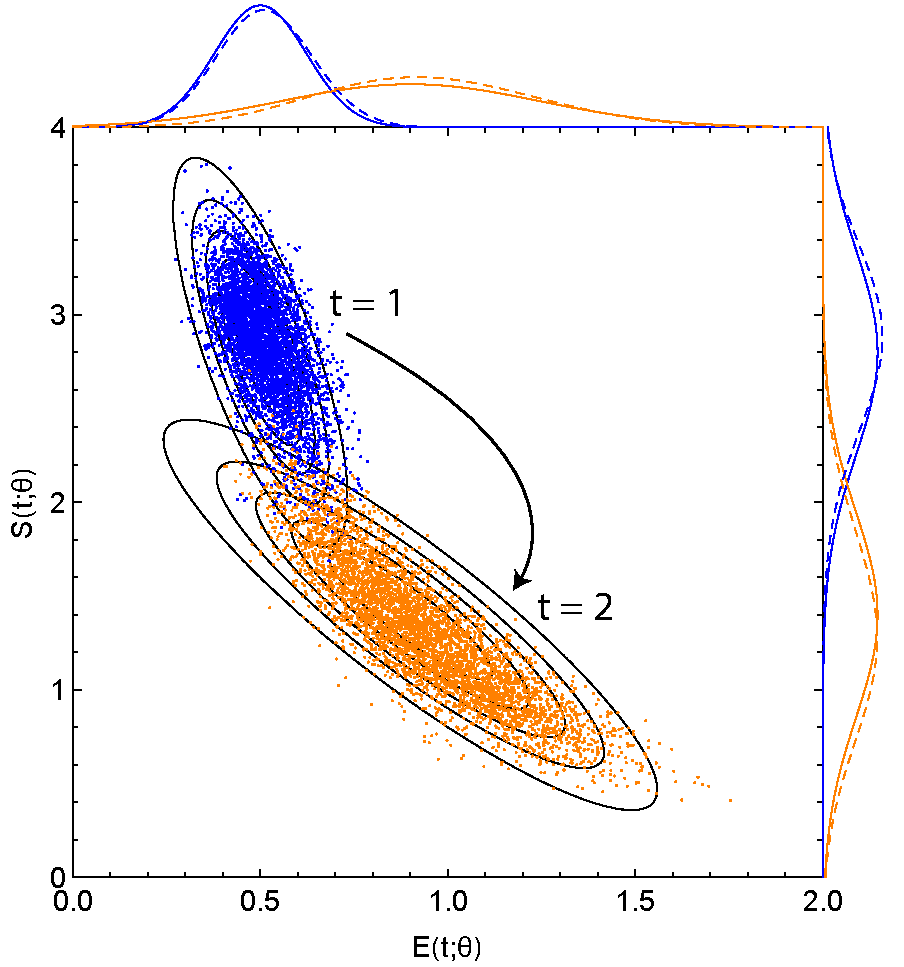
\includegraphics[width=0.65\textwidth]{../figures/mm_4d_outputs.pdf}}
  \caption{\textbf{Michaelis-Menten model. Posterior output samples from CMC (coloured points) versus contour plots (black solid lines) of the joint marginal distributions of eq. (\ref{eq:MM_4d_output}).} Enzyme and substrate measurements are given by the horizontal and vertical axes, respectively. Output functionals for $(q_1,q_2)$ and $(q_3,q_4)$ are given by blue and orange points, respectively. The solid and dashed coloured lines outside the panels indicate exact target marginals of eq. (\ref{eq:MM_4d_output}) and those estimated by CMC, respectively. In the ``ContourVolumeEstimator'' step, 200,000 independent samples were used, and in the MCMC step, 10,000 samples across each of 4 Markov chains were used, with the first half of the chains discarded as ``warm-up'' \cite{lambert2018Student}. Mathematica's ``SmoothKernelDistribution'' function, using Gaussian kernels \cite{mathematica} and bandwidths ranging from 0.1 to 0.4, was used to reconstruct marginal densities.}
  \label{fig:mm_4d_outputs}
\end{figure}


\subsection{TNF signalling pathway}
We now illustrate how CMC can be applied to an ODE system of larger size: the tumour necrosis factor (TNF) signalling pathway model introduced in \cite{chaves2008bistable} and used by \cite{hasenauer2011identification} to illustrate a Bayesian approach to cell population variability estimation. The model incorporates known activating and inhibitory interactions between four key species within the TNF pathway: active caspase 8, $x_1$, active caspase 3, $x_2$, a nuclear transcription factor, $x_3$ and its inhibitor, $x_4$, such that
%
\begin{equation}\label{eq:tnf}
\begin{aligned}
\frac{dx_1}{dt} &= -x_1(t) + \frac{1}{2}\left[\beta_4(x_3(t))\alpha_1(u(t)) + \alpha_3(x_2(t))\right]\\
\frac{dx_2}{dt} &= -x_2(t) + \alpha_2(x_1(t)) \beta_3(x_3(t))\\
\frac{dx_3}{dt} &= -x_3(t) + \beta_2(x_2(t)) \beta_5(x_4(t))\\
\frac{dx_4}{dt} &= -x_4(t) + \frac{1}{2}\left[\beta_1(u(t)) + \alpha_4(x_3(t))\right],
\end{aligned}
\end{equation}
%
with initial conditions,
\begin{equation}
x_1(0)=0.0, \quad x_2(0)=0.0, \quad x_3(0)=0.29, \quad x_4(0)=0.625.
\end{equation}
%which correspond to the steady state of the system when $x_2=0$.
The functions $\alpha_i$ and $\beta_j$ represent activating and inhibitory interactions respectively,
%
\begin{equation}
\begin{aligned}
\alpha_i(z) &= \frac{z^2}{a_i^2 + z^2}, \quad i=1, \dots, 4,\\
\beta_j(z)  &= \frac{b_j^2}{b_j^2 + z^2}, \quad j = 1, \dots, 5,
\end{aligned}
\end{equation}
%
and the parameters $a_i$ for $i\in(1,2,3,4)$ and $b_j$ for $j\in(1,2,3,4,5)$ represent activation and inhibition thresholds. The function $u(t)$ represents a TNF stimulus represented by a top hat function,
%
\begin{equation}
u(t)=\begin{cases}
1, & \text{if $t\in[0,2]$}.\\
0, & \text{otherwise}.
\end{cases}
\end{equation}
%

\subsubsection{Recovering parameter values in under-determined systems}
In under-determined models, a set of parameters of non-zero volume can produce the same output values. A consequence of this unidentifiability is that we cannot perform ``full circle'' inference: that is, using a known parameter distribution to generate an output distribution does not result in that parameter distribution being recovered through inference. We illustrate this idea by generating an output distribution by varying a single parameter value between runs of the forward model \eqref{eq:tnf} and performing inference on all nine system parameters, whilst collecting only two output measurements. Specifically, we randomly sample $a_1\sim \mathcal{N}(0.6, 0.05)$ for each simulation of the forward model, whilst holding the other parameters constant, $$(a_2,a_3,a_4,b_1,b_2,b_3,b_4,b_5)=(0.2, 0.2, 0.5, 0.4, 0.7, 0.3, 0.5, 0.4),$$ and measure $q_1=x_1(2.0)$ and $q_2=x_2(1.0)$ in each case. In doing so, we obtain an output distribution well-approximated by the bivariate Gaussian distribution,
%
\begin{equation}\label{eq:tnf_circular_target}
\begin{aligned}
\boldsymbol{q} = \begin{pmatrix} q_1 \\ q_2 \end{pmatrix}
&=
\begin{pmatrix}
x_1(2.0)\\
x_2(1.0)\\
\end{pmatrix} \\
&\sim  \mathcal{N}
\begin{bmatrix}
\begin{pmatrix}
0.26\\
0.07\\
\end{pmatrix}, \;\;
\begin{pmatrix}
2.1\times 10^{-4} & 5.9\times 10^{-5}\\
5.9\times 10^{-5} & 1.8\times 10^{-5}\\
\end{pmatrix}
\end{bmatrix}.
\end{aligned}
\end{equation}
%
We now apply CMC to the target output distribution given by eq. (\ref{eq:tnf_circular_target}) to estimate a posterior distribution over all nine parameters of eq. (\ref{eq:tnf}). Apart from a few cases, the priors for each parameter were chosen to \emph{exclude} the values that were used to generate the output distribution (see Table \ref{tab:priors}), to illustrate how the recovered posterior distribution and data generating distribution differ. In Figure \ref{fig:tnf_circular_versus}A, we plot the actual parameter values (horizontal axis) used to generate the data versus the estimated values (vertical axis). This illustrates that, due to the chosen priors, there is a disjunction between actual and estimated parameter values in all cases apart from $a_1$. Though because the model is under-determined, the corresponding output distribution closely approximates the target despite these differences (Figure \ref{fig:tnf_circular_versus}B).


\begin{figure}[H]
\centerline{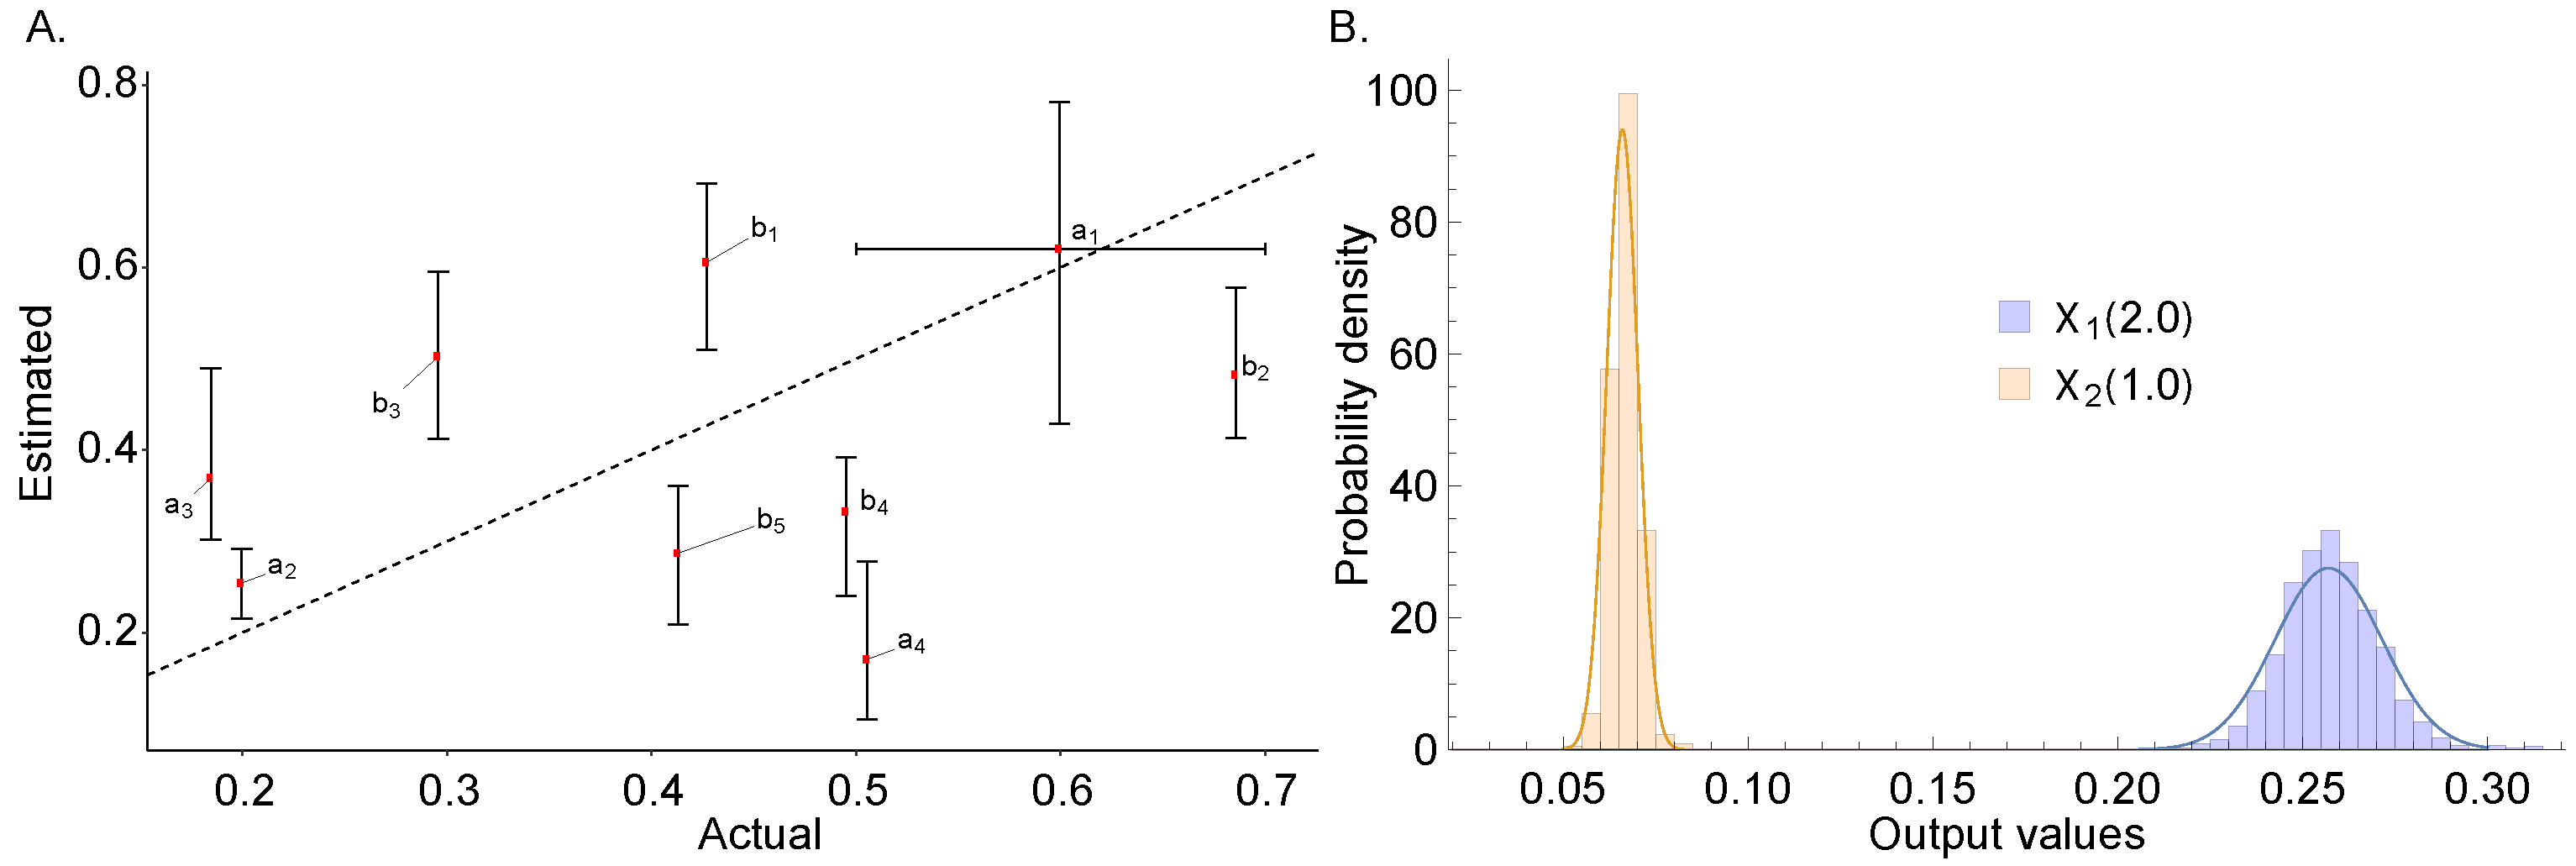
\includegraphics[width=1.0\textwidth]{../figures/tnf_circular_both.pdf}}
\caption{\textbf{TNF signalling pathway model. (A) Actual parameter values versus estimated quantiles for the output distribution of eq. (\ref{eq:tnf_circular_target}). (B) Marginal output targets (solid lines) and sampled output distributions (\textcolor{blue}{dashed} lines).} In A, in the vertical direction, red points indicate 50\% posterior quantiles and upper and lower whiskers indicate 97.5\% and 2.5\% quantiles, respectively; in the horizontal direction, with the exception of $a_1$, red points indicate the parameter values used to generate the data; for $a_1$, the red point indicates the mean of the Gaussian distribution used to generate the data and the whiskers indicate its 95\% quantiles. In CMC, 10,000 independent samples were used in the ``ContourVolumeEstimator'' step, and 5,000 MCMC samples across each of 4 Markov chains were used in the second, with the first half of the chains discarded as ``warm-up'' \cite{lambert2018Student}. \textcolor{blue}{Mathematica's ``SmoothKernelDistribution'' function, using a Gaussian kernel \cite{mathematica} and a bandwidth of 0.003 was used to reconstruct marginal densities.}}
	\label{fig:tnf_circular_versus}
\end{figure}

\subsubsection{Bimodal output distribution}

The dynamics of all cells can often be modelled by assuming cells exist in subpopulation clusters, which evolve differently over time. A hint that such subpopulation structure may exist is output distributions with multiple modes. We now apply CMC to investigate a bimodal output distribution for the TNF signalling pathway model similar to that investigated by \cite{hasenauer2011identification}. We aim to estimate the posterior parameter distribution mapping to the following output distribution,
%
\begin{equation}
\boldsymbol{q} = \begin{pmatrix} q_1 \\ q_2 \\ q_3 \end{pmatrix},
\end{equation}
where,
\begin{equation}
\begin{aligned}
q_1 = \boldsymbol{x}_2(1.0) &\sim \mathcal{N}(0.06, 0.01)\\
q_2 = \boldsymbol{x}_2(2.0) &\sim\frac{1}{2}\left(\mathcal{N}(0.1, 0.01) + \mathcal{N}(0.14, 0.01)\right)\\
q_3 = \boldsymbol{x}_2(4.0) &\sim\frac{1}{2}\left(\mathcal{N}(0.1, 0.01) + \mathcal{N}(0.20, 0.01)\right),\\
\end{aligned}
\end{equation}
%
where the target distributions for $\boldsymbol{q}_2(2.0)$ and $\boldsymbol{q}_2(4.0)$ indicate mixtures of univariate Gaussians, and the priors used are given in Table \ref{tab:priors}. This target distribution, along with the unique trajectories obtained by applying the CMC algorithm, are shown in Figure \ref{fig:tnf_samples_vs_distribution}. This figure illustrates that a bimodal output distribution causes CMC to sample clusters of parameter values, without the need for subpopulation information to be provided ahead of estimation.

\begin{figure}[H]
	\centerline{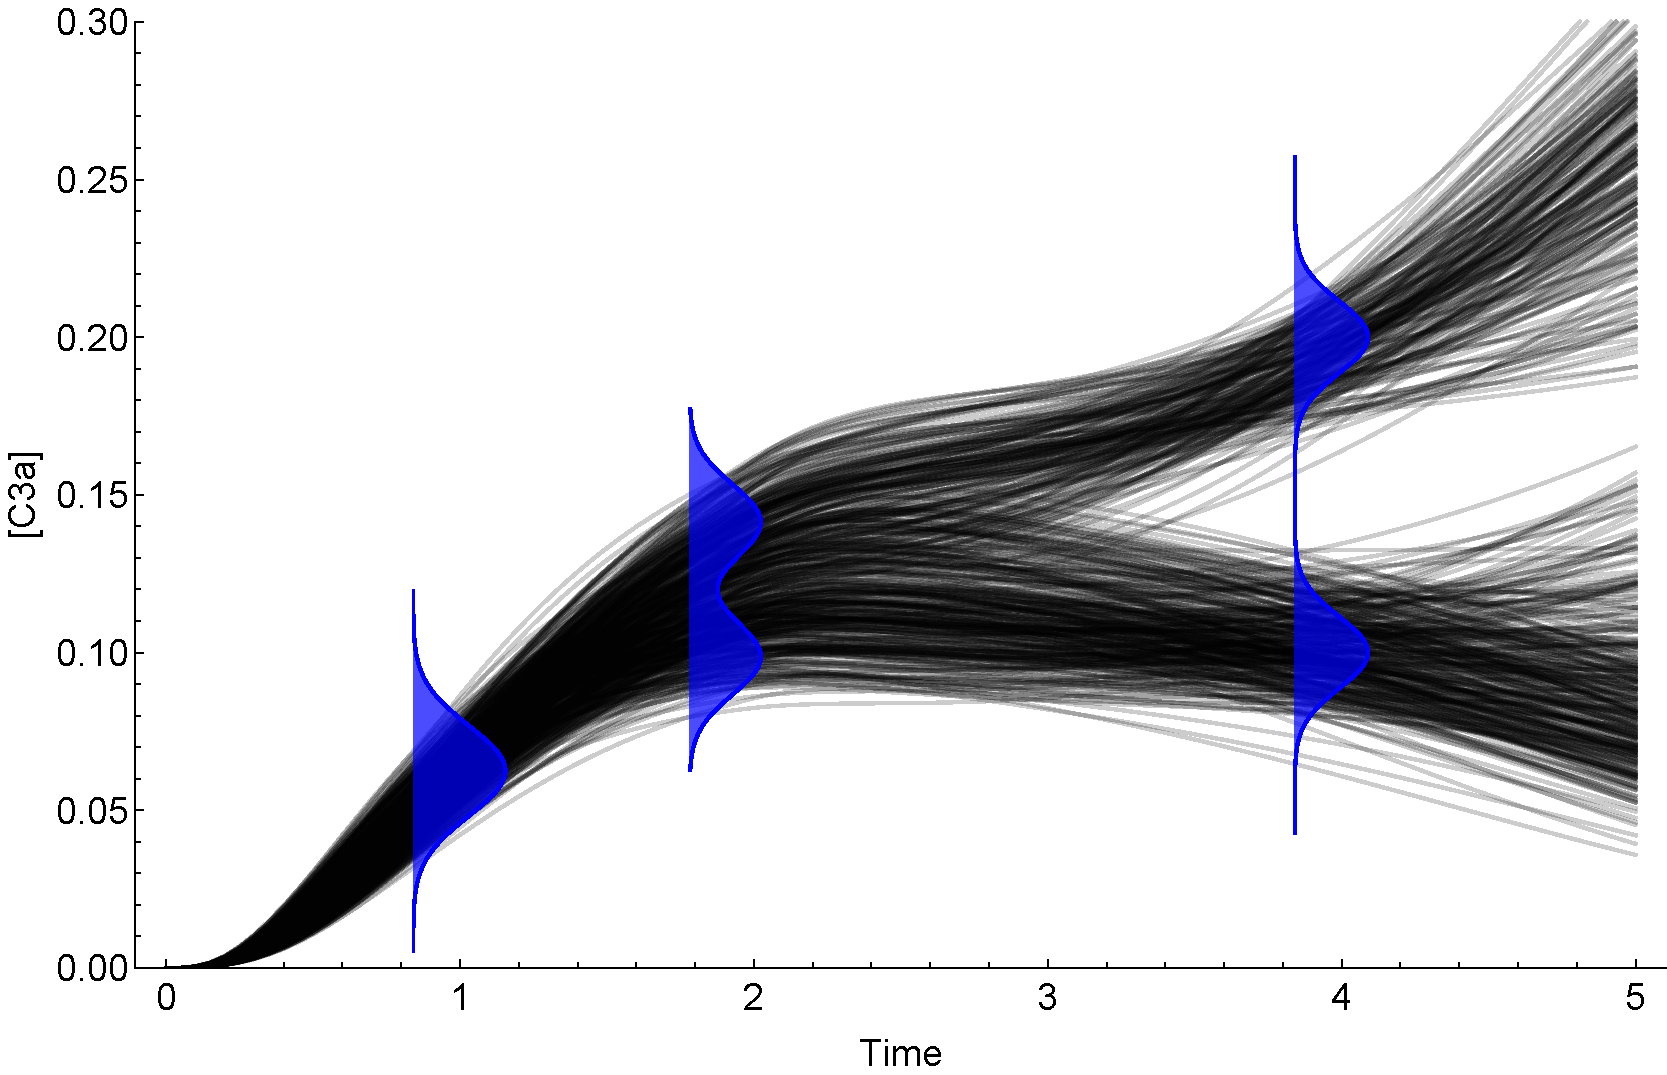
\includegraphics[width=0.8\textwidth]{../figures/tnf_samples_vs_distribution.pdf}}
	\caption{\textbf{TNF signalling pathway model. Target output distribution (dashed plots with grey filling) and unique trajectories (black solid lines) obtained from the posterior parameter distribution.} In CMC, 10,000 independent samples were used in the ``ContourVolumeEstimator'' step, and 5,000 MCMC samples across each of 4 Markov chains were used in the second, with the first half of the chains discarded as ``warm-up'' \cite{lambert2018Student}.}
	\label{fig:tnf_samples_vs_distribution}
\end{figure}

\begin{table}[H]
\centering
%\scriptsize
\begin{adjustwidth}{0in}{0in}%
\begin{tabularx}{1.0\textwidth}{llclcc}
Model	& Target  & Parameter & Prior    & Prior  & Prior  \\
        & density &           & density  & $p_1$  & $p_2$  \\
\toprule
Growth  & 2D     & $R_T$       & uniform & $2.5 \times 10^5$ &  $8 \times 10^5$\\
factor  & Gaussian & $k_1$       & uniform & 0.25 & 3.0\\
                && $k_{-1}$    & uniform & 2.0 & 20.0\\
                && $k_{deg}$   & uniform & 0.005 & 0.03\\
                && $k^*_{deg}$ & uniform & 0.1 & 0.5\\
\toprule
Growth  & 2D     & $R_T$ & Gaussian & $5 \times 10^5$ &  $1 \times 10^5$\\
factor  & Gaussian & $k_1$ & Gaussian & 0.5 & 0.1\\
                && $k_{-1}$ & Gaussian & 3.0 & 1.0\\
                && $k_{deg}$ & Gaussian & 0.02 & 0.005\\
                && $k^*_{deg}$ & Gaussian & 0.3 & 0.1\\
\toprule
Michaelis- & bimodal  & $k_f$ & uniform & 0.2 &  15\\
Menten     & Gaussian   & $k_r$ & uniform & 0.2 & 2.0\\
&& $k_{cat}$ & uniform & 0.5 & 3.0\\
\toprule
Michaelis- & 4D    & $k_f$ & uniform & 0.2 &  15\\
Menten     & Gaussian& $k_r$ & uniform & 0.2 & 2.0\\
&& $k_{cat}$ & uniform & 0.2 & 3.0\\
&& $E_0$ & uniform & 3.0 & 5.0\\
&& $S_0$ & uniform & 5.0 & 10.0\\
&& $C_0$ & uniform & 0.0 & 0.2\\
&& $P_0$ & uniform & 0.0 & 0.2\\
\toprule
TNF & bivariate & $a_1$ & uniform & 0.4 & 0.8\\
signalling & Gaussian& $a_2$ & uniform & 0.1 & 0.7\\
&& $a_3$ & uniform & 0.3 & 0.7\\
&& $a_4$ & uniform & 0.1 & 0.3\\
&& $b_1$ & uniform & 0.5 & 0.7\\
&& $b_2$ & uniform & 0.4 & 0.6\\
&& $b_3$ & uniform & 0.4 & 0.6\\
&& $b_4$ & uniform & 0.2 & 0.4\\
&& $b_5$ & uniform & 0.2 & 0.4\\
\toprule
TNF  & bimodal  & $a_1$ & uniform & 0.5 & 0.7\\
signalling& Gaussian & $a_2$ & uniform & 0.1 & 0.3\\
&& $a_3$ & uniform & 0.1 & 0.3\\
&& $a_4$ & uniform & 0.4 & 0.6\\
&& $b_1$ & uniform & 0.3 & 0.5\\
&& $b_2$ & uniform & 0.6 & 0.8\\
&& $b_3$ & uniform & 0.2 & 0.4\\
&& $b_4$ & uniform & 0.4 & 0.6\\
&& $b_5$ & uniform & 0.3 & 0.5\\
\end{tabularx}
\caption{\textbf{Priors used for each example in \S\ref{sec:results}.} The parameters $p_1$ and $p_2$ indicate the prior hyperparameters: for uniform priors, these correspond to the lower and upper limits; for Gaussian priors, they correspond to the mean and standard deviation.}
\label{tab:priors}
\end{adjustwidth}
\end{table}
